\chapter*{Target of evaluation} 
\label{target_of_eval}
\addcontentsline{toc}{chapter}{Target of evaluation}

This work aims at producing an assessment of the procedures that interest the process of uploading and aggregating the Dutch election results. More specifically, we want to analyze the processes of inputting the election results of the commonalities, uploading such results to a centralized server, and computing and approving the aggregated result of the election.

To do so, some assumption had to be made. As can be seen in figure \ref{fig:map} the following was assumed:

\begin{itemize}
    \item the authentication process is split in a first-party 2FA service, and in a third-party MFA service, depending on the user role.
    \item the third-party MFA service has access to the private WAN via VPN tunneling.
    \item The used VPN is a third-party service.
    \item The private WAN is relying on a third-party ISP infrastructure.
\end{itemize}

\begin{figure}[h!]
    \centering
    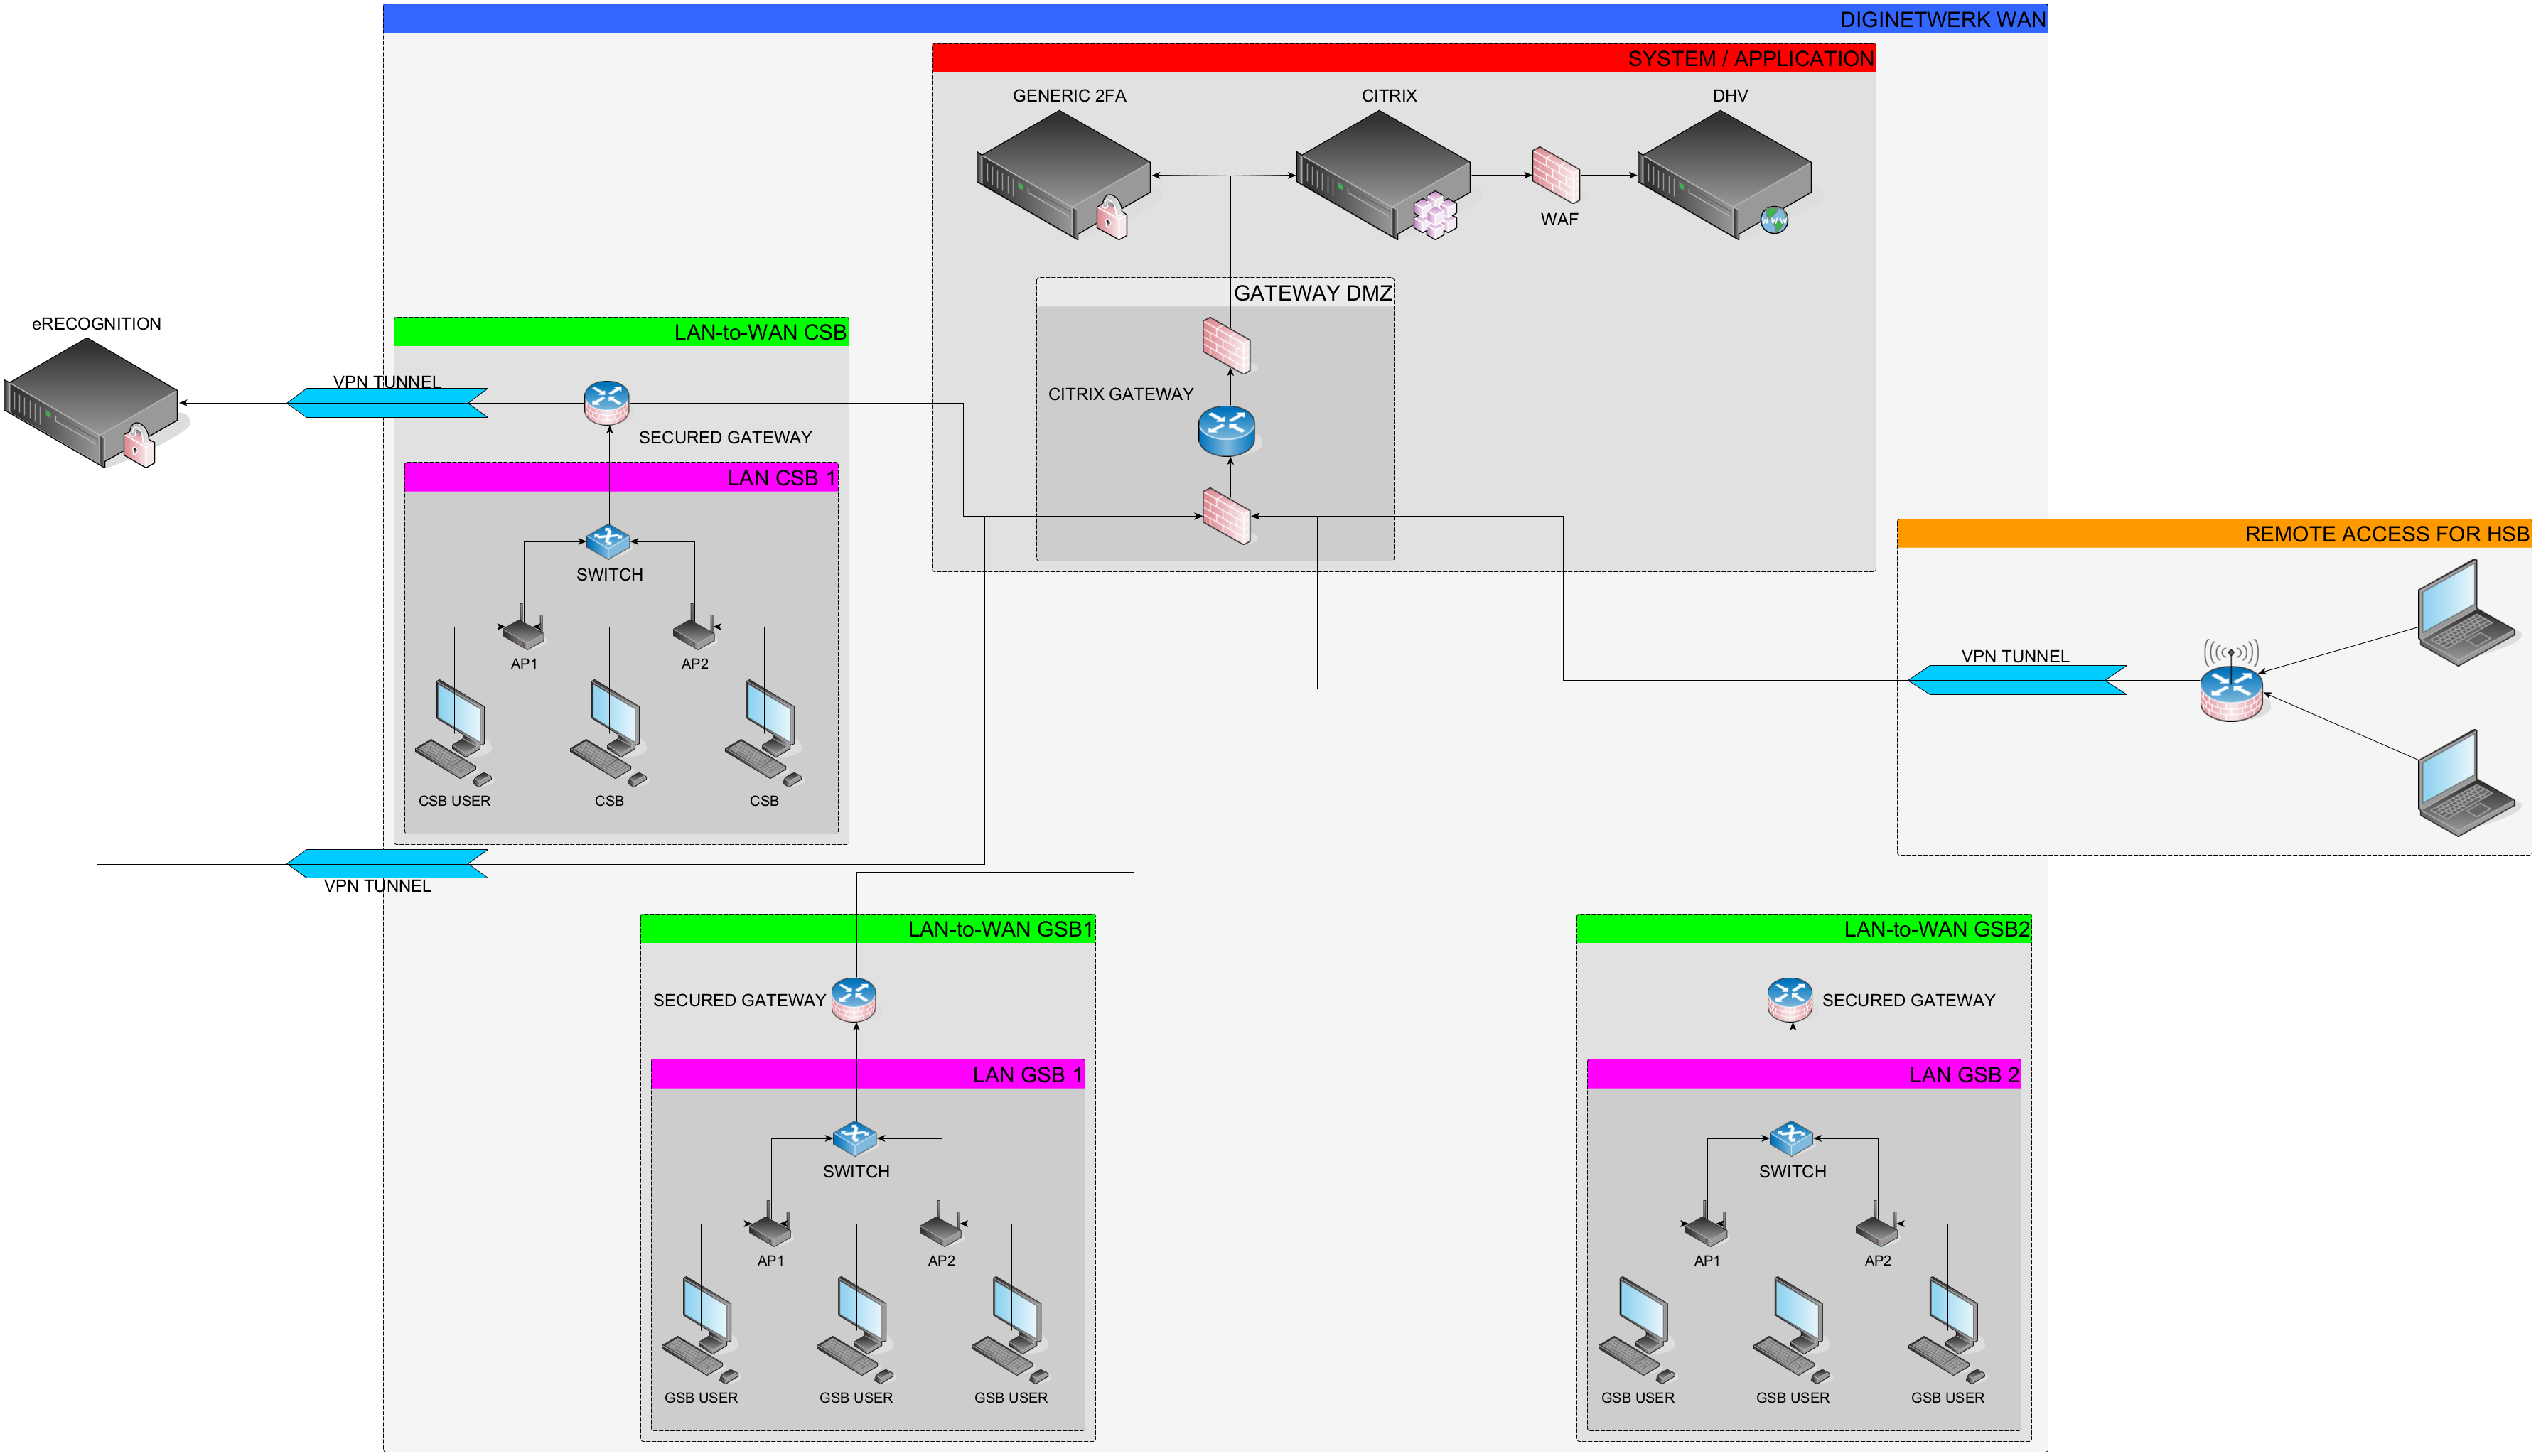
\includegraphics[keepaspectratio,width=1\textwidth]{01-target/img/map.png}
    \caption{High-level assumed network topology}
    \label{fig:map}
\end{figure}